% little trick to replace lib.tex by this
\renewcommand{\doctitle}[1]{
	\chapter{#1}
}
\renewcommand{\biblio}[1]{}
\doctitle{Dimensionnement du modulateur sigma-delta}

\subsection{Fonctionnement et théorie}
<<<<<<< HEAD
Le schéma bloc du modulateur sigma-delta se trouve
à la figure \ref{fig:sigma-delta-schema-blocs}. Le
modulateur du synthétiseur utilise une bascule asymétrique.
=======
Le schéma bloc du modulateur sigma-delta est représenté
à la figure \ref{fig:sigma-delta-schema-blocs}. 
>>>>>>> c92f779ff2b4f8bd1e35ffa2a415b08368b407d9

\begin{figure}[ht]
	\centering
	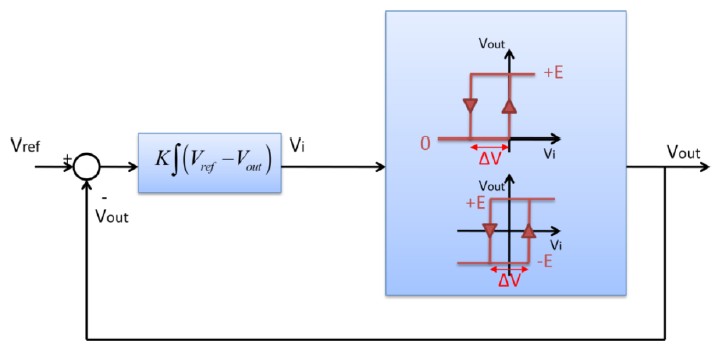
\includegraphics[scale=0.75]{img/schema-blocs.png}
	\caption{Schéma bloc du modulateur sigma-delta.}
	\label{fig:sigma-delta-schema-blocs}
\end{figure}

<<<<<<< HEAD
La période d'oscillation du signal de sortie (qui est 
identique à la période d'oscillation du signal intermédiaire
$V_I$ sur la figure \ref{fig:sigma-delta-schema-blocs}).
se calcule en effectuant le raisonnement suivant.

Initialement, soit $V_{\text{ref}}$  positif et
$V_{\text{out}} = 0$. $V_I$ est alors immédiatement positif
et $V_{\text{out}}$ sature directement à $E$. Comme $V_{\text{ref}}$
est $\leq E$, $V_I$ va maintenant décroître jusqu'à atteindre
$\Delta V$. A ce moment précis, $V_{\text{out}} = 0$
et donc $V_I$ va croître jusqu'à atteindre 0, et ainsi de suite.

De là s'obtiennent le temps de descente $t_f$ et le temps de montée $t_r$
du signal $V_I$\footnote{Ce signal sera soit un signal triangulaire,
soit un signal en dents de scie, selon la valeur de $V_{\text{ref}}$.}
=======
Considérons le cas de la bascule asymétrique.
Dans un premier temps, calculons la période
d'oscillation de la sortie (qui est identique
à la période d'oscillation de $V_I$ sur la figure
\ref{fig:sigma-delta-schema-blocs}.

Nous démarrons avec un signal $V_{\text{ref}}$ positif et
$V_{\text{out}} = 0$. $V_I$ est alors immédiatement positif
et $V_{\text{out}}$ sature directement à $E$. Comme $V_{\text{ref}}$
est $\leq E$, $V_I$ va maintenant décroître jusqu'à atteindre
$\Delta V$. A ce moment précis, nous aurons à nouveau $V_{\text{out}} = 0$
et donc $V_I$ va croître jusqu'à atteindre 0, et ainsi de suite.

Sur base de cela, nous pouvons facilement calculer
le temps de descente $t_f$ et le temps de montée $t_r$
du signal $V_I$\footnote{Ce signal sera soit un signal triangulaire,
soit un signal en dents de scie, selon la valeur de $V_{\text{ref}}$.}.
Nous trouvons facilement,
>>>>>>> c92f779ff2b4f8bd1e35ffa2a415b08368b407d9
\[ t_f = -\frac{\Delta V}{(V_{\text{ref}} - E)K},\]
\[ t_r = \frac{\Delta V}{KV_{\text{ref}}}.\]

La période $T$ étant la somme du temps de descente et du temps
<<<<<<< HEAD
de montée, elle est donnée par
\[ T = \frac{\Delta V}{K}\left(\frac{1}{V_{\text{ref}}} - \frac{1}{V_{\text{ref}} - E}\right) \]
=======
de montée, nous trouvons
\[ T = \frac{\Delta V}{K}\left(\frac{1}{V_{\text{ref}}} - \frac{1}{V_{\text{ref}} - E}\right)\]
>>>>>>> c92f779ff2b4f8bd1e35ffa2a415b08368b407d9
et donc finalement
\begin{equation} 
	f = -\frac{K}{\Delta V} \frac{V_{\text{ref}}(V_{\text{ref}}-E)}{E}.
	\label{eq:sigma-delta-frequency}
\end{equation}

\paragraph{Remarque}
A partir du temps de descente et du temps de montée, nous
pouvons prouver que la moyenne du signal carré $V_{\text{out}}$
vaut bien $V_{\text{ref}}$. Il suffit de démontrer l'égalité
suivante
\[ \frac{E \cdot t_f + 0 \cdot t_r}{T} = V_{\text{ref}}.\]

La fréquence en fonction de $V_{\text{ref}}$ est donc
une parabole avec une racine en \unit{0}{\volt} et une
racine en \unit{E}{\volt}.

<<<<<<< HEAD
La fréquence de sortie maximale est atteinte pour 
=======
Nous pouvons déduire plusieurs chose de l'équation \ref{eq:sigma-delta-frequency}. 
Premièrement, la fréquence de sortie maximale est atteinte pour 
>>>>>>> c92f779ff2b4f8bd1e35ffa2a415b08368b407d9
$V_{\text{ref}} = \frac{E}{2}$ et vaut
\[ f_{\text{max}} = \frac{K}{\Delta V}\frac{E}{4}. \]
Ensuite, pour un signal $V_{\text{ref}}$ sinusoïdal dont
l'amplitude peut être négative, la fréquence sature.
Or, dans le cas du synthétiseur, le signal $V_{\text{ref}}$
est la sortie de notre VCO (après passage dans un filtre pour
en extraire une sinusoïdale pure).
Il faudra donc ``déplacer'' la parabole de manière à ce qu'elle soit
centrée autour de l'origine.

\subsection{Dimensionnement et circuit réel}
Le circuit du modulateur sigma-delta est représenté
à la figure \ref{fig:sigma-delta-circuit}.

\begin{figure}[ht]
	\centering
	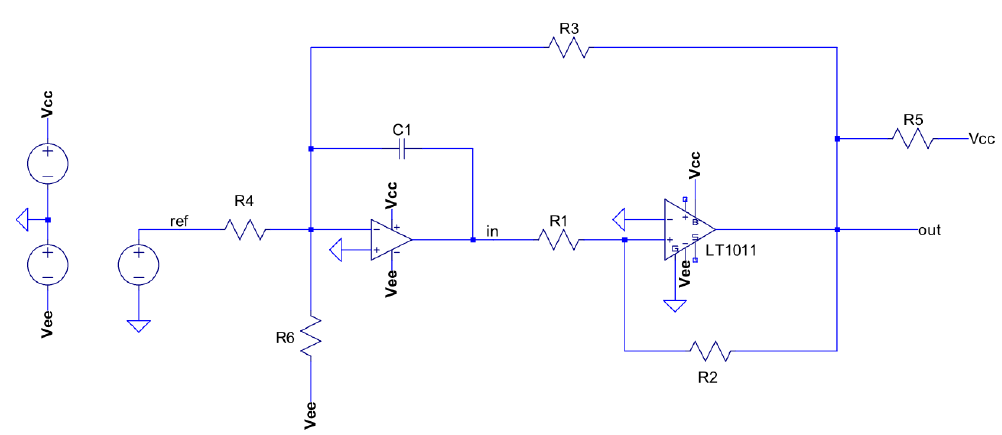
\includegraphics[scale=0.7]{img/sigma-delta-circuit.png}
	\caption{Circuit du modulateur.}
	\label{fig:sigma-delta-circuit}
\end{figure}

<<<<<<< HEAD
La résolution de ce circuit permet d'obtenir des équations
de la même forme que celles de la figure
\ref{fig:sigma-delta-schema-blocs}.

L'amplificateur opérationnel étant connecté en contre-réaction,
sa bornée d'entrée est virtuellement à la masse : $v_- = v_+ = 0$.
Les différents courants dans le circuit sont alors donnés par
=======
Nous allons résoudre ce circuit pour obtenir des équations
de la même forme que celles de la figure
\ref{fig:sigma-delta-schema-blocs}.
Concentrons nous d'abord sur l'amplificateur
opérationnel. Grâce à la boucle de contre
réaction négative, nous pouvons dire $v_- = v_+ = 0$.
Nous obtenons ensuite  les courants suivants:
>>>>>>> c92f779ff2b4f8bd1e35ffa2a415b08368b407d9
\[ i_{R_4} = \frac{V_{\text{ref}}}{R_4},\]
\[ i_{R_6} = \frac{V_{\text{ee}}}{R_6},\]
\[ i_{R_3} = \frac{V_{\text{out}}}{R_3},\]
\[ i_{C_1} = -C_1\fdif{v_{\text{in}}}{t}.\]
<<<<<<< HEAD
KCL permet ensuite d'écrire l'équation suivante
\[ i_{C_1} = i_{R_4} + i_{R_6} + i_{R_3}\]
et donc d'obtenir
=======
Appliquons ensuite KCL et  écrivons
\[ i_{C_1} = i_{R_4} + i_{R_6} + i_{R_3}.\]
De cette relation, nous tirons
>>>>>>> c92f779ff2b4f8bd1e35ffa2a415b08368b407d9
\[ v_{\text{in}} = -\frac{1}{C_1}\int \frac{V_{\text{ref}}}{R_4}
+ \frac{V_{\text{ee}}}{R_6} + \frac{V_{\text{out}}}{R_3}.\]

Pour se ramener à l'équation de la figure
<<<<<<< HEAD
\ref{fig:sigma-delta-schema-blocs}, on
=======
\ref{fig:sigma-delta-schema-blocs}, nous posons
>>>>>>> c92f779ff2b4f8bd1e35ffa2a415b08368b407d9
$V'_{\text{ref}} = -R_3(\frac{V_{\text{ref}}}{R_4}+\frac{V_{\text{ee}}}{R_6})$
pour enfin obtenir
\[ v_{\text{in}} = \frac{1}{C_1R_3} \int V'_{\text{ref}} - V_{\text{out}}\]
où $V'_{\text{ref}}$ correspond au $V_{\text{ref}}$
de la figure \ref{fig:sigma-delta-schema-blocs}.

<<<<<<< HEAD
Pour dimensionner le modulateur, plusieurs contraintes doivent
être respectées. Premièrement la fréquence maximale doit être
de \unit{80}{\kilo\hertz}. Et deuxièment, la parabole doit s'étendre
de manière à ce que ces racines soient \unit{-15}{\volt} et
\unit{+15}{\volt}. Enfin, $\Delta V$ doit être choisit de manière
à ce que la bascule ne soit pas sensible au bruit.
=======
Pour dimensionner le modulateur, nous devons respecter plusieurs
contraintes. Premièrement, la fréquence pour $V_{\text{ref}} =$
\unit{7.5}{\volt} doit être de \unit{80}{\kilo\hertz}. Et deuxièment,
nous devons déplacer la parabole
de manière à ce que ces racines soient \unit{-15}{\volt} et
\unit{+15}{\volt}. Enfin, nous devons choisir $\Delta V$ de manière
à ce que la bascule ne soit pas sensible au bruit (quelques millivolts).
>>>>>>> c92f779ff2b4f8bd1e35ffa2a415b08368b407d9

Nous allons directement anticiper une non-idéalité de la bascule,
la valeur de saturation $E$ n'est pas égale à la tension
d'alimention. Nous avons plutôt $E \approx$ \unit{13.5}{\volt}.

Pour centrer la parabole, il faut que $\frac{R_3}{R_6}V_{\text{ee}}$
soit égale à \unit{6.75}{\volt}. Il faut ensuite étirer la
parabole de manière à ce que ses racines soient $\pm$\unit{15}{\volt}.
Il faut donc $\frac{R_3}{R_4} = 0.45$. 

En utilisant des valeurs de composants standards (série de Renard E12), 
nous pouvons choisir, $R_3 =$ \unit{22}{\kilo\ohm} et $R_4 = R_6 =
$ \unit{48.5}{\kilo\ohm}.

Passons ensuite à la contrainte sur la fréquence. Nous avons la 
relation suivante:
\[ \frac{K}{\Delta V}\frac{E}{4} = 80000.\]
Nous pouvons fixer arbitrairemet $\Delta V$ à \unit{1}{\volt}. Nous avons alors
$K = \frac{1}{C_1R_3} = 23703.7037$ et donc $C1 =$ \unit{1.9}{\nano\farad}.
Enfin, comme $\Delta V = \frac{R_1}{R_2}E$, nous pouvons par exemple
choisir $R_1 =$ \unit{10}{\kilo\ohm} et $R_2 =$ \unit{134.6}{\kilo\ohm}.

% TODO : on peut sans doute réaliser encore un meilleur
% dimensionnement en considérant dans les calculs les valeurs
% exactes (je veux dire par là les valeurs mesurées sur circuit,
% pas les valeurs théoriques).

Pour appliquer la signal de sortie du modulateur
à l'étage suivant du circuit, il faudra utiliser un diviseur
résistif car l'étage suivant ne supporte pas des entrées supérieures
à \unit{5}{\volt}.

\subsection{Confrontation des mesures et de la théorie}
En superposant le graphe théorique que nous pouvons obtenir avec les valeurs
obtenues dans la section précédente
et des mesures effectuées sur une implémentation en circuit
du modulateur, nous obtenons la figure \ref{fig:sigma-delta-f-vs-vref-dim-vs-real}.

\begin{figure}[ht]
	\centering
	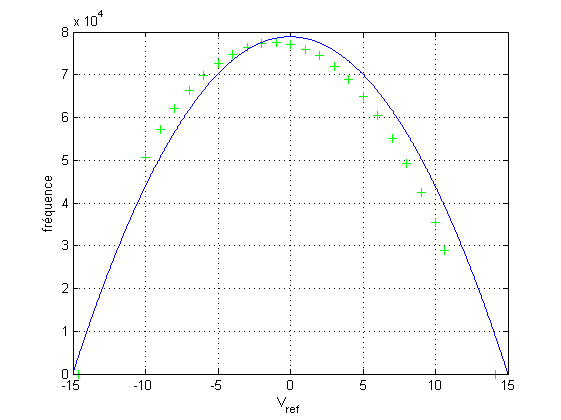
\includegraphics[scale=0.7]{img/sigma-delta-f-vs-vref-dim-vs-real.png}
	\caption{En bleu, les prévisions théoriques et en vert les mesures.}
	\label{fig:sigma-delta-f-vs-vref-dim-vs-real}
\end{figure}

Nous constatons que la théorie colle assez bien à la réalité. Le
faible décalage dépend sans doute des tolérances des résistances,
des variations dans les alimentations (le MyDAQ sort, dans ce cas, du
\unit{+14.10}{\volt} et du \unit{-14.62}{\volt} plutôt que du
$\pm$\unit{15}{\volt}), des variations dans la valeur de saturation
$E$ ($\approx$ \unit{13.62}{\volt}). Nous pourrions effectuer un
dimensionnement plus précis à partir de ces valeurs réelles afin
d'obtenir une prévision théorique encore plus proche de la réalité.
% FIXME (à confirmer)
Le problème, c'est que les valeurs des tensions
d'alimentation (par exemple) dépendent justement de la charge 
connectée, et donc du choix des résistances effectuées lors du dimensionnement.

\end{document}
